\documentclass[../SpecificaTecnica.tex]{subfiles}
\begin{document}
	\section{Componenti e classi principali}
		\subsection{SWEDesigner}
				I package contenuti al suo interno sono:
				\begin{itemize}
					\item SWEDesigner::Client;
					\item SWEDesigner::Server.
				\end{itemize}
				Questo package non contiene delle classi.
			\subsection{SWEDesigner::Client}
				% IMMAGINE ARCHITETTURA CLIENT GENERALE
				\begin{figure}[H]\label{fig:ClientSubsystem}
					\centering
					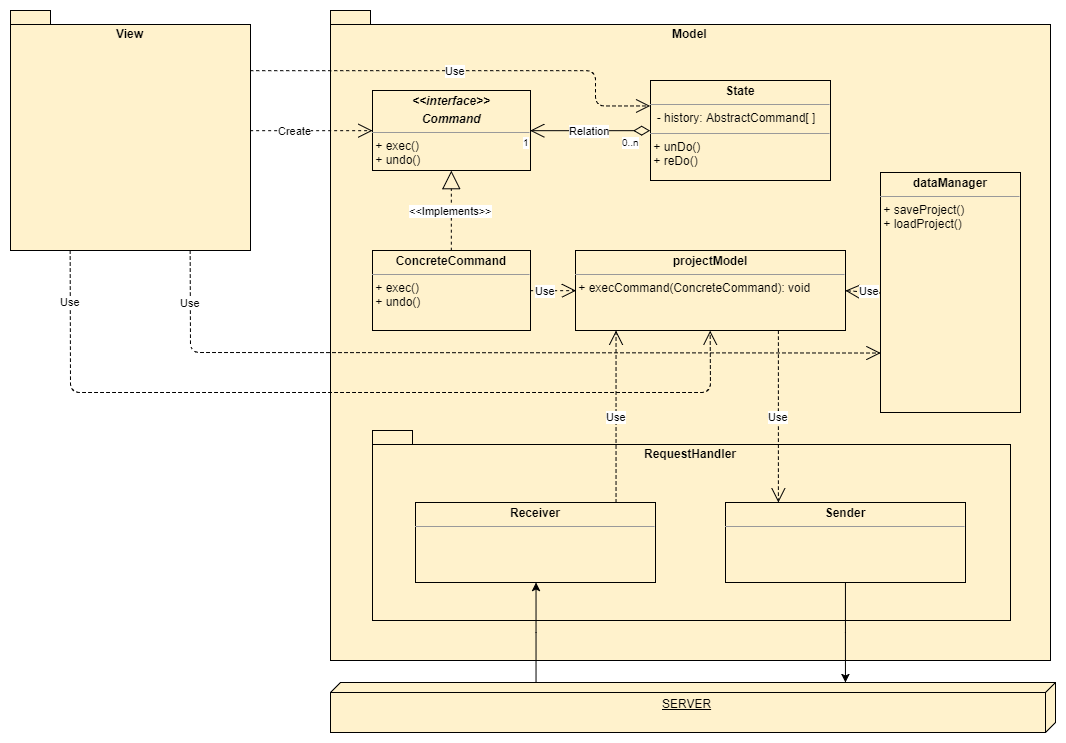
\includegraphics[scale=0.46]{Immagini/DiagrammaArchitettura/ClientSubsystem.png}
					\caption{Architettura del client}
				\end{figure}
				I package contenuti al suo interno sono:
				\begin{itemize}
					\item SWEDesigner::Client::Model;
					\item SWEDesigner::Client::View.
				\end{itemize}
				Questo package non contiene delle classi.
			\subsection{SWEDesigner::Client::Model}
				\hypertarget{SWEDesigner::Client::Model}
				I package contenuti al suo interno sono:
				\begin{itemize}
					\item SWEDesigner::Client::Model::Items.
				\end{itemize}
				Le classi contenute al suo interno verranno elencate qui di seguito.

				\subsubsection{SWEDesigner::Client::Model::DataManager}
				\hypertarget{SWEDesigner::Client::Model::DataManager}{}
					\begin{itemize}
						\item \textbf{Tipo}: \emph{Classe statica};
						\item \textbf{Descrizione}: Si occupa della persistenza dei dati, in particolare del salvataggio su file system locale del progetto già esistente.\\;
						\item \textbf{Relazioni con le altre classi}:
						\begin{itemize}
							\item OUT \hyperlink{SWEDesigner::Client::Model::ProjectModel}{\emph{SWEDesigner::Client::Model::ProjectModel}}: si occupa di gestire la parte logica dell'editor;
							\item OUT \hyperlink{SWEDesigner::Client::Model::Project}{\emph{SWEDesigner::Client::Model::Project}}: si occupa di gestire gli elementi contenuti nel diagramma.
						\end{itemize}
					\end{itemize}

				\subsubsection{SWEDesigner::Client::Model::ProjectModel}
				\hypertarget{SWEDesigner::Client::Model::ProjectModel}{}
					% IMMAGINE ARCHITETTURA MAINMODEL
					\begin{figure}[H]\label{fig:Model}
						\centering
						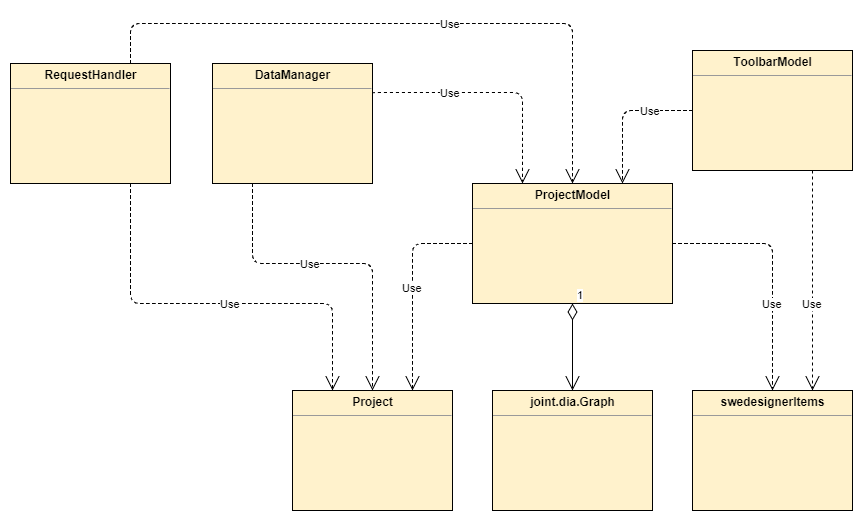
\includegraphics[scale=0.46]{Immagini/DiagrammaArchitettura/MainModel.png}
						\caption{Architettura di Model}
					\end{figure}

					\begin{itemize}
						\item \textbf{Tipo}: \emph{Classe};
						\item \textbf{Descrizione}: Model del progetto corrente. Si occupa di gestire il graph (joint.dia.Graph) e tutti gli eventi ad esso associati;
						\item \textbf{Relazioni con le altre classi}:
						\begin{itemize}
							\item IN \hyperlink{SWEDesigner::Client::Model::DataManager}{\emph{SWEDesigner::Client::Model::DataManager}}: si occupa della persistenza dei dati, in particolare del salvataggio su file system locale del progetto e del caricamento di un progetto già esistente;
							\hyperlink{SWEDesigner::Client::Model::ToolbarModel}{\emph{SWEDesigner::Client::Model::ToolbarModel}}: È il componente del programma che si occupa di gestire la parte logica della toolbar;
							\item IN \hyperlink{SWEDesigner::Client::Model::RequestHandler}{\emph{SWEDesigner::Client::Model::RequestHandler}}: si occupa di gestire i dati ricevuti dal server;
							\item OUT \hyperlink{SWEDesigner::Client::Model::Project}{\emph{SWEDesigner::Client::Model::Project}}: si occupa di gestire gli elementi contenuti nel diagramma;
							\item OUT \hyperlink{SWEDesigner::Client::Model::Items::Swedesigner}{\emph{SWEDesigner::Client::Model::Items::Swedesigner}}: è il contenitore degli elementi che si possono inserire in un diagramma.
						\end{itemize}
					\end{itemize}

				\subsubsection{SWEDesigner::Client::Model::ToolbarModel}
				\hypertarget{SWEDesigner::Client::Model::ToolbarModel}{}
					\begin{itemize}
						\item \textbf{Tipo}: \emph{Classe};
						\item \textbf{Descrizione}: È il componente del programma che si occupa di gestire la parte logica della toolbar;
						\item \textbf{Relazioni con le altre classi}:
						\begin{itemize}
							\item OUT \hyperlink{SWEDesigner::Client::Model::ProjectModel}{\emph{SWEDesigner::Client::Model::ProjectModel}}: si occupa di gestire la parte logica dell'editor;
							\item OUT \hyperlink{SWEDesigner::Client::Model::Items::Swedesigner}{\emph{SWEDesigner::Client::Model::Items::Swedesigner}}: è il contenitore degli elementi che si possono inserire in un diagramma.
						\end{itemize}
					\end{itemize}

				\subsubsection{SWEDesigner::Client::Model::Project}
				\hypertarget{SWEDesigner::Client::Model::Project}{}
					\begin{itemize}
						\item \textbf{Tipo}: \emph{Classe};
						\item \textbf{Descrizione}: Contenitore di tutti gli elementi del progetto correntemente aperto nella Single Page Application;
						\item \textbf{Relazioni con le altre classi}:
						\begin{itemize}
							\item IN \hyperlink{SWEDesigner::Client::Model::ProjectModel}{\emph{SWEDesigner::Client::Model::ProjectModel}}: si occupa di gestire la parte logica dell'editor;
							\item IN \hyperlink{SWEDesigner::Client::Model::DataManager}{\emph{SWEDesigner::Client::Model::DataManager}}: si occupa della persistenza dei dati, in particolare del salvataggio su file system locale del progetto e del caricamento di un progetto già esistente;
							\item IN \hyperlink{SWEDesigner::Client::Model::RequestHandler}{\emph{SWEDesigner::Client::Model::RequestHandler}}: si occupa di gestire i dati ricevuti dal server;
						\end{itemize}
					\end{itemize}
				
				\subsubsection{SWEDesigner::Client::Model::RequestHandler}
				\hypertarget{SWEDesigner::Client::Model::RequestHandler}{}
					\begin{itemize}
						\item \textbf{Tipo}: \emph{Classe};
						\item \textbf{Descrizione}: Si occupa della gestione delle comunicazioni tra client e server (lato client);
						\item \textbf{Relazioni con le altre classi}:
						\begin{itemize}
							\item OUT \hyperlink{SWEDesigner::Client::Model::ProjectModel}{\emph{SWEDesigner::Client::Model::ProjectModel}}: si occupa di gestire la parte logica dell'editor;
							\item OUT \hyperlink{SWEDesigner::Client::Model::Project}{\emph{SWEDesigner::Client::Model::Project}}: si occupa di gestire gli elementi contenuti nel diagramma.
						\end{itemize}
					\end{itemize}

			\subsection{SWEDesigner::Client::View}
				\hypertarget{SWEDesigner::Client::View}{}
				È il componente del programma che si occupa di gestire l'interfaccia grafica. Nella particolare declinazione MVC adottata da Backbone.js, si occupa anche di gestire gli input dell'utente.
				% IMMAGINE ARCHITETTURA VIEW
					\begin{figure}[H]\label{fig:View}
						\centering
						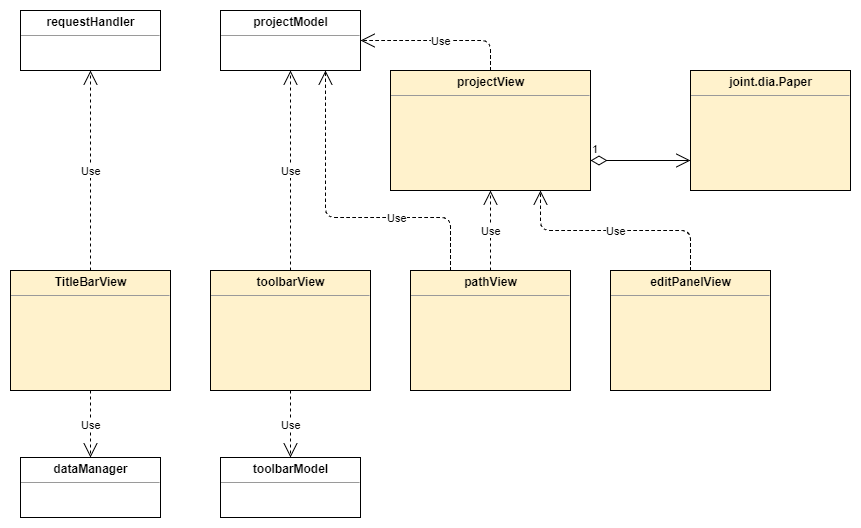
\includegraphics[scale=0.44]{Immagini/DiagrammaArchitettura/View.png}
						\caption{Architettura di View}
					\end{figure}
				Questo package non contiene dei sottopackage.
				Le classi contenute al suo interno verranno elencate qui di seguito.

				\subsubsection{SWEDesigner::Client::View::ProjectView}
					\hypertarget{SWEDesigner::Client::View::ProjectView}{}
					\begin{itemize}
						\item \textbf{Tipo}: \emph{Class};
						\item \textbf{Descrizione}: Questa classe gestisce il diagramma disegnato e le interazioni dell'utente con esso;
						\item \textbf{Relazioni con le altre classi}:
						\begin{itemize}
							\item IN \hyperlink{SWEDesigner::View::PathView}{\emph{PathView}}: gestisce l'interfaccia grafica della barra di indirizzo;
							\item IN \hyperlink{SWEDesigner::View::EditPanelView}{\emph{EditPanelView}}: gestisce l'interfaccia grafica del pannello di editing.
							\item OUT \hyperlink{SWEDesigner::Model::ProjectModel}{\emph{ProjectModel}}: si occupa di gestire la parte logica dell'editor;
							\item OUT joint.dia.Paper: gestisce l'interfaccia grafica dell'area dei diagrammi.
						\end{itemize}
					\end{itemize}
					
				\subsubsection{SWEDesigner::Client::View::TitlebarView}
					\hypertarget{SWEDesigner::Client::View::TitlebarView}{}
					\begin{itemize}
						\item \textbf{Tipo}: \emph{Class};
						\item \textbf{Descrizione}: È il componente del programma che fa la funzione di view per la barra del titolo, dove saranno collocati il menu dell’applicazione e gli shortcut;
						\item \textbf{Relazioni con le altre classi}:
						\begin{itemize}
							\item OUT \hyperlink{SWEDesigner::Model::RequestHandler}{\emph{RequestHandler}}: gestisce la comunicazione con il server;
							\item OUT \hyperlink{SWEDesigner::Model::DataManager}{\emph{DataManager}}: gestisce la persistenza dei dati su file system.
						\end{itemize}
					\end{itemize}

				\subsubsection{SWEDesigner::Client::View::ToolbarView}
					\hypertarget{SWEDesigner::Client::View::ToolbarView}{}
					\begin{itemize}
						\item \textbf{Tipo}: \emph{Class};
						\item \textbf{Descrizione}: È il componente del programma che fa la funzione di view per la toolbar dove saranno collocati gli strumenti per editare i diagrammi;
						\item \textbf{Relazioni con le altre classi}:
						\begin{itemize}
							\item OUT \hyperlink{SWEDesigner::Model::ProjectModel}{\emph{ProjectModel}}: si occupa di gestire la parte logica dell'editor;
							\item OUT \hyperlink{SWEDesigner::Model::ToolbarModel}{\emph{ToolbarModel}}: si occupa di gestire la parte logica della toolbar.
						\end{itemize}
					\end{itemize}

				\subsubsection{SWEDesigner::Client::View::PathView}
					\hypertarget{SWEDesigner::Client::View::PathView}{}
					\begin{itemize}
						\item \textbf{Tipo}: \emph{Class};
						\item \textbf{Descrizione}: È il componente del programma che fa la funzione di view per il cosiddetto breadcrumb dove viene inserita la posizione corrente;
						\item \textbf{Relazioni con le altre classi}:
						\begin{itemize}
							\item OUT \hyperlink{SWEDesigner::Model::ProjectModel}{\emph{ProjectModel}}: si occupa di gestire la parte logica dell'editor;
							\item OUT \hyperlink{SWEDesigner::View::ProjectView}{\emph{ProjectView}}: si occupa di gestire la parte grafica del model.
						\end{itemize}
					\end{itemize}

				\subsubsection{SWEDesigner::Client::View::EditPanelView}
					\hypertarget{SWEDesigner::Client::View::EditPanelView}{}
					\begin{itemize}
						\item \textbf{Tipo}: \emph{Class};
						\item \textbf{Descrizione}: ;
						\item \textbf{Relazioni con le altre classi}:
						\begin{itemize}
							\item OUT \hyperlink{SWEDesigner::View::ProjectView}{\emph{ProjectView}}: si occupa di gestire la parte grafica del model.
						\end{itemize}
					\end{itemize}

			\subsection{SWEDesigner::Server}
			% IMMAGINE ARCHITETTURA SERVER GENERALE
			\begin{figure}[H]\label{fig:ServerSubsystem}
				\centering
				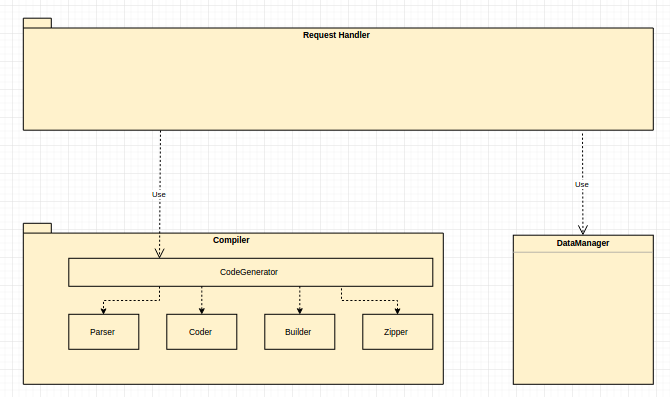
\includegraphics[scale=0.4]{Immagini/DiagrammaArchitettura/ServerSubsystem.png}
				\caption{Architettura del server}
			\end{figure}
			I package contenuti al suo interno sono:
			\begin{itemize}
				\item SWEDesigner::Server::CodeGenerator;
				\item SWEDesigner::Server::DAORequestHandler;
				\item SWEDesigner::Server::RequestHandler.
			\end{itemize}
			Questo package non contiene delle classi.
			
			\subsection{SWEDesigner::Server::CodeGenerator}
			I package contenuti al suo interno sono:
			\begin{itemize}
				\item SWEDesigner::Server::CodeGenerator::Builder;
				\item SWEDesigner::Server::CodeGenerator::Coder;
				\item SWEDesigner::Server::CodeGenerator::Parser;
				\item SWEDesigner::Server::CodeGenerator::Zipper.
			\end{itemize}
			Le classi contenute al suo interno verranno elencate qui di seguito.
			
			\subsubsection{SWEDesigner::Server::CodeGenerator::CodeGenerator}
			\hypertarget{SWEDesigner::Server::CodeGenerator::CodeGenerator}{}
			\begin{itemize}
				\item \textbf{Tipo}: \emph{Class};\\
				\item \textbf{Descrizione}: Rende disponibile la funzionalità per cui, dato un file in formato JSON che contiene le informazioni necessarie a codificare un programma, restituisce un pacchetto in formato .zip contenente i file del codice sorgente che costituiscono il programma rappresentato dal file in input. I file prodotti sono organizzati in packages, come indicato nel file JSON in input;\\
				\item \textbf{Relazioni con le altre classi:}
				\begin{itemize}
					\item OUT \hyperlink{SWEDesigner::Server::CodeGenerator::Parser::Parser}{\emph{SWEDesigner::Server::CodeGenerator::Parser::Parser}}
					\item OUT \hyperlink{SWEDesigner::Server::CodeGenerator::Coder::JavaCoder}{\emph{SWEDesigner::Server::CodeGenerator::Coder::JavaCoder}}
					\item OUT \hyperlink{SWEDesigner::Server::CodeGenerator::Coder::JavascriptCoder}{\emph{SWEDesigner::Server::CodeGenerator::Coder::JavascriptCoder}}
					\item OUT \hyperlink{SWEDesigner::Server::CodeGenerator::Builder::Builder}{\emph{SWEDesigner::Server::CodeGenerator::Builder::Builder}}
					\item OUT \hyperlink{SWEDesigner::Server::CodeGenerator::Zipper::Zipper}{\emph{SWEDesigner::Server::CodeGenerator::Zipper::Zipper}}
					\item IN \hyperlink{SWEDesigner::Server::RequestHandler::RequestHandler}{\emph{SWEDesigner::Server::RequestHandler::RequestHandler}}
				\end{itemize}	
			\end{itemize}
			
				
			
			
			%%%%%%%%%%%%%%%%%%%%%%%%%%%%%%%%%%%%%%%%%%%%%%%%%%%%%%%%%%%%%%%%%%%%%%%%%%%%%%%%%%%%%%%%%%%%%%%%%%%%%%%%%%%%%%%%%%%%%%%%%%%%%%%%%%%%%%%%%%%%%%%%%%%%%%%%%%%%%%%%%%%%%%%%
			
			\subsection{SWEDesigner::Server::CodeGenerator::Parser}
			Questo package non contiene dei sottopackage.
			Le classi contenute al suo interno verranno elencate qui di seguito.
			
			\subsubsection{SWEDesigner::Server::CodeGenerator::Parser::Parser}
			\hypertarget{SWEDesigner::Server::CodeGenerator::Parser::Parser}{}
			\begin{itemize}
				\item \textbf{Tipo}: \emph{Class};
				\item \textbf{Descrizione}: Rende disponibile la funzionalità, dato un file JSON valido in input, di ottenere un oggetto contenente le informazioni che costituiscono il file JSON di input;
				\item \textbf{Relazioni con le altre classi:}
				\begin{itemize}
					\item IN \hyperlink{SWEDesigner::Server::CodeGenerator::CodeGenerator}{\emph{SWEDesigner::Server::CodeGenerator::CodeGenerator}}
				\end{itemize}	
			\end{itemize}
			
			%%%%%%%%%%%%%%%%%%%%%%%%%%%%%%%%%%%%%%%%%%%%%%%%%%%%%%%%%%%%%%%%%%%%%%%%%%%%%%%%%%%%%%%%%%%%%%%%%%%%%%%%%%%%%%%%%%%%%%%%%%%%%%%%%%%%%%%%%%%%%%%%%%%%%%%%%%%%%%%%%%%%%%%%
			
			
			\subsection{SWEDesigner::Server::CodeGenerator::Coder}
			% IMMAGINE ARCHITETTURA CODER
			\begin{figure}[H]\label{fig:Coder}
				\centering
				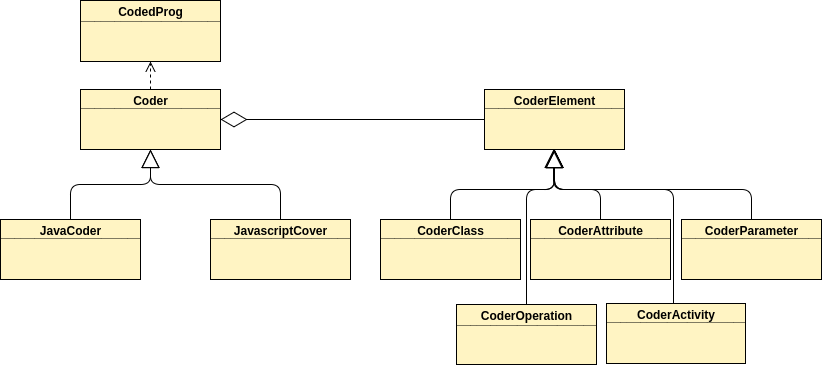
\includegraphics[scale=0.46]{Immagini/DiagrammaArchitettura/Coder.png}
				\caption{Architettura di Coder}
			\end{figure}
			
			Questo package non contiene dei sottopackage.\\
			Le classi contenute al suo interno verranno elencate qui di seguito.
			
			%		\subsubsection{SWEDesigner::Server::CodeGenerator::Coder::Coder}
			%		Componente che funge da interfaccia alle operazioni di codifica di una stringa, in formato JSON che rappresenta un programma valido; tali operazioni permettono di ottenere un %	oggetto contenente il codice sorgente, in Java o Javascript, corrispondente alla stringa in input.\\
			%		FAN-IN:
			%		\begin{itemize}
			%			\item JavaCoder: si occupa di trasformare un oggetto JSON ricevuto in input in un oggetto contenente il codice sorgente scritto in java;
			%			\item JavaScriptCoder: si occupa di trasformare un oggetto JSON ricevuto in input in un oggetto contenente il codice sorgente scritto in javascript.
			%		\end{itemize}
			%		FAN-OUT:
			%			\item CoderElement: componente astratto che offre la funzionalità che permette di associare ad ogni stringa contenuta nel file JSON il corrispondente codice sorgente.
			%		\end{itemize}
			
			\subsubsection{SWEDesigner::Server::CodeGenerator::Coder::JavaCoder}
			\hypertarget{SWEDesigner::Server::CodeGenerator::Coder::JavaCoder}{}
			\begin{itemize}
				\item \textbf{Tipo}: \emph{Class};
				\item \textbf{Descrizione}: Rende disponibile la funzionalità, dato un oggetto in input che che contiene le informazioni necessarie a codificare un programma, di ottenere un oggetto contenente il codice sorgente, in linguaggio Java, corrispondente all'oggetto in input;
				\item \textbf{Relazioni con le altre classi:}
				\begin{itemize}
					\item IN \hyperlink{SWEDesigner::Server::CodeGenerator::CodeGenerator}{\emph{SWEDesigner::Server::CodeGenerator::CodeGenerator}}
				\end{itemize}	
			\end{itemize}
			
			\subsubsection{SWEDesigner::Server::CodeGenerator::Coder::JavascriptCoder}
			\hypertarget{SWEDesigner::Server::CodeGenerator::Coder::JavascriptCoder}{}
			\begin{itemize}
				\item \textbf{Tipo}: \emph{Class};
				\item \textbf{Descrizione}: Rende disponibile la funzionalità, dato un oggetto in input che contiene le informazioni necessarie a codificare un programma, di ottenere un oggetto contenente il codice sorgente, in linguaggio Javascript, corrispondente all'oggetto in input;
				\item \textbf{Relazioni con le altre classi:}
				\begin{itemize}
					\item IN \hyperlink{SWEDesigner::Server::CodeGenerator::CodeGenerator}{\emph{SWEDesigner::Server::CodeGenerator::CodeGenerator}}
				\end{itemize}	
			\end{itemize}
			
			
			%		\subsubsection{SWEDesigner::Server::CodeGenerator::Coder::CoderClass}
			%		È il componente che mette a disposizione la funzionalità, data una stringa in input in formato JSON che rappresenta una classe valida, di ottenere il corrispondente codice %		sorgente di tale classe.\\
			%		Non ci sono dipendenze IN.\\
			%		FAN-OUT:
			%		\begin{itemize}
			%			\item CoderElement: componente astratto che offre la funzionalità che permette di associare ad ogni stringa contenuta nel file JSON il corrispondente codice sorgente.
			%		\end{itemize}
			
			\subsubsection{SWEDesigner::Server::CodeGenerator::Coder::CoderOperation}
			\hypertarget{SWEDesigner::Server::CodeGenerator::Coder::CoderOperation}{}
			\begin{itemize}
				\item \textbf{Tipo}: \emph{Class};
				\item \textbf{Descrizione}: Rende disponibile la funzionalità che permette di codificare l'intestazione dell'operazione corrispondente al contenuto dell'oggetto operationObj di input;
				\item \textbf{Relazioni con le altre classi:}
				\begin{itemize}
					\item IN \hyperlink{SWEDesigner::Server::CodeGenerator::Coder::JavascriptCoder}{\emph{SWEDesigner::Server::CodeGenerator::Coder::JavascriptCoder}}
					\item IN \hyperlink{SWEDesigner::Server::CodeGenerator::Coder::JavaCoder}{\emph{SWEDesigner::Server::CodeGenerator::Coder::JavaCoder}}
				\end{itemize}	
			\end{itemize}
			
			
			
			\subsubsection{SWEDesigner::Server::CodeGenerator::Coder::CoderParameter}
			\hypertarget{SWEDesigner::Server::CodeGenerator::Coder::CoderParameter}{}
			\begin{itemize}
				\item \textbf{Tipo}: \emph{Class};
				\item \textbf{Descrizione}: Rende disponibile la funzionalità che permette di codificare un parametro, corrispondente al contenuto dell'oggetto parameterObj di input;
				\item \textbf{Relazioni con le altre classi:}
				\begin{itemize}
					\item IN \hyperlink{SWEDesigner::Server::CodeGenerator::Coder::JavascriptCoder}{\emph{SWEDesigner::Server::CodeGenerator::Coder::JavascriptCoder}}
					\item IN \hyperlink{SWEDesigner::Server::CodeGenerator::Coder::JavaCoder}{\emph{SWEDesigner::Server::CodeGenerator::Coder::JavaCoder}}
				\end{itemize}	
			\end{itemize}
			
			
			\subsubsection{SWEDesigner::Server::CodeGenerator::Coder::CoderAttribute}
			\hypertarget{SWEDesigner::Server::CodeGenerator::Coder::CoderAttribute}{}
			\begin{itemize}
				\item \textbf{Tipo}: \emph{Class};
				\item \textbf{Descrizione}: Rende disponibile la funzionalità che permette di codificare un attributo corrispondente al contenuto dell'oggetto attributeObj di input;
				\item \textbf{Relazioni con le altre classi:}
				\begin{itemize}
					\item IN \hyperlink{SWEDesigner::Server::CodeGenerator::Coder::JavascriptCoder}{\emph{SWEDesigner::Server::CodeGenerator::Coder::JavascriptCoder}}
					\item IN \hyperlink{SWEDesigner::Server::CodeGenerator::Coder::JavaCoder}{\emph{SWEDesigner::Server::CodeGenerator::Coder::JavaCoder}}
				\end{itemize}	
			\end{itemize}
			
			
			
			\subsubsection{SWEDesigner::Server::CodeGenerator::Coder::CoderActivity}
			\hypertarget{SWEDesigner::Server::CodeGenerator::Coder::CoderActivity}{}
			\begin{itemize}
				\item \textbf{Tipo}: \emph{Class};
				\item \textbf{Descrizione}: Rende disponibile la funzionalità che permette di codificare l'implementazione di un'operazione, corrispondente al contenuto dell'oggetto activityObj di input; 
				\item \textbf{Relazioni con le altre classi:}
				\begin{itemize}
					\item IN \hyperlink{SWEDesigner::Server::CodeGenerator::Coder::JavascriptCoder}{\emph{SWEDesigner::Server::CodeGenerator::Coder::JavascriptCoder}}
					\item IN \hyperlink{SWEDesigner::Server::CodeGenerator::Coder::JavaCoder}{\emph{SWEDesigner::Server::CodeGenerator::Coder::JavaCoder}}
				\end{itemize}	
			\end{itemize}
			
			
			\subsubsection{SWEDesigner::Server::CodeGenerator::Coder::CodedProg}
			\hypertarget{SWEDesigner::Server::CodeGenerator::Coder::CodedProg}{}
			\begin{itemize}
				\item \textbf{Tipo}: \emph{Class};
				\item \textbf{Descrizione}: È il componente che contiene il codice sorgente prodotto dal Coder; 
				\item \textbf{Relazioni con le altre classi:}
				\begin{itemize}
					\item IN \hyperlink{SWEDesigner::Server::CodeGenerator::Coder::JavascriptCoder}{\emph{SWEDesigner::Server::CodeGenerator::Coder::JavascriptCoder}}
					\item IN \hyperlink{SWEDesigner::Server::CodeGenerator::Coder::JavaCoder}{\emph{SWEDesigner::Server::CodeGenerator::Coder::JavaCoder}}
				\end{itemize}	
			\end{itemize}
			
			%%%%%%%%%%%%%%%%%%%%%%%%%%%%%%%%%%%%%%%%%%%%%%%%%%%%%%%%%%%%%%%%%%%%%%%%%%%%%%%%%%%%%%%%%%%%%%%%%%%%%%%%%%%%%%%%%%%%%%%%%%%%%%%%%%%%%%%%%%%%%%%%%%%%%%%%%%%%%%%%%%%%%%%%
			
			\subsection{SWEDesigner::Server::CodeGenerator::Builder}
			Questo package non contiene dei sottopackage.\\
			Le classi contenute al suo interno verranno elencate qui di seguito.
			
			
			\subsubsection{SWEDesigner::Server::CodeGenerator::Builder::Builder}
			\hypertarget{SWEDesigner::Server::CodeGenerator::Builder::Builder}{}
			\begin{itemize}
				\item \textbf{Tipo}: \emph{Class};
				\item \textbf{Descrizione}: Rende disponibile la funzionalità che permette di creare su disco la directory contenente il programma corrispondente all'oggetto program di tipo CodedProgram; 
				\item \textbf{Relazioni con le altre classi:}
				\begin{itemize}
					\item IN \hyperlink{SWEDesigner::Server::CodeGenerator::CodeGenerator}{\emph{SWEDesigner::Server::CodeGenerator::CodeGenerator}}
				\end{itemize}	
			\end{itemize}
			
			
			
			%%%%%%%%%%%%%%%%%%%%%%%%%%%%%%%%%%%%%%%%%%%%%%%%%%%%%%%%%%%%%%%%%%%%%%%%%%%%%%%%%%%%%%%%%%%%%%%%%%%%%%%%%%%%%%%%%%%%%%%%%%%%%%%%%%%%%%%%%%%%%%%%%%%%%%%%%%%%%%%%%%%%%%%%
			
			
			\subsection{SWEDesigner::Server::CodeGenerator::Zipper}
			Questo package non contiene dei sottopackage.\\
			Le classi contenute al suo interno verranno elencate qui di seguito.
			
			\subsubsection{SWEDesigner::Server::CodeGenerator::Zipper::Zipper}
			\hypertarget{SWEDesigner::Server::CodeGenerator::Builder::Builder}{}
			\begin{itemize}
				\item \textbf{Tipo}: \emph{Class};
				\item \textbf{Descrizione}: Rende disponibile la funzionalità che permette di creare un pacchetto in formato zip della directory specificata in input; \\
				\item \textbf{Relazioni con le altre classi:}
				\begin{itemize}
					\item IN \hyperlink{SWEDesigner::Server::CodeGenerator::CodeGenerator}{\emph{SWEDesigner::Server::CodeGenerator::CodeGenerator}}
				\end{itemize}	
			\end{itemize}
			
			
			\subsection{SWEDesigner::Server::DAO}
			Questo package non contiene dei sottopackage.\\
			Le classi contenute al suo interno verranno elencate qui di seguito.
			\subsubsection{SWEDesigner::Server::DAO::DAO}
			\hypertarget{SWEDesigner::Server::DAO::DAO}{}
			\begin{itemize}
				\item \textbf{Tipo}: \emph{Class};
				\item \textbf{Descrizione}: Espone le funzionalità che permettono di interagire con il database delle bubbles; \\
				\item \textbf{Relazioni con le altre classi:}
				\begin{itemize}
					\item IN \hyperlink{SWEDesigner::Server::RequestHandler::RequestHandler}{\emph{SWEDesigner::Server::CodeGenerator::CodeGenerator}}
				\end{itemize}	
			\end{itemize}
			
			
			\subsection{SWEDesigner::Server::RequestHandler}
			Questo package non contiene dei sottopackage.\\
			Le classi contenute al suo interno verranno elencate qui di seguito
			
			\subsection{SWEDesigner::Server::RequestHandler}::RequestHandler
			\hypertarget{SWEDesigner::Server::RequestHandler::RequestHandler}{}
			\begin{itemize}
				\item \textbf{Tipo}: \emph{Class};
				\item \textbf{Descrizione}: Espone le funzionalità che permettono di interagire con il database delle bubbles; \\
				\item \textbf{Relazioni con le altre classi:}
				\begin{itemize}
					\item IN \hyperlink{SWEDesigner::Client::Model::RequestHandler}{\emph{SWEDesigner::Client::Model::RequestHandler}}
				\end{itemize}	
			\end{itemize}
\end{document}
